\documentclass[12pt, letter-paper]{article}
\usepackage[utf8]{inputenc}
\usepackage{graphicx}
\usepackage{fancyhdr}
\usepackage{float}
\newcommand{\comment}[1]{}

\title{Math 189R Final Writeup}
\author{Andy Liu, Justin Jiang}
\date{July 2020}

\begin{document}

\maketitle

\section{Introduction}

The upcoming 2020 U.S. Presidential Election will be one of the most important events in the year, and as such, the competition between incumbent Donald Trump and Democratic Nominee and former Vice-President Joe Biden has attracted substantial amounts of news coverage. Media opinions have also had an increasingly high effect on the election results in recent years, with Hillary Clinton going as far as to claim that media coverage was a significant factor in her 2016 loss to Trump.

As such, our project uses text sentiment analysis and topic modeling to analyze media coverage of the 2020 U.S. Presidential Election. We further refined this by the usage of topic modeling to consider media coverage of the U.S. Presidential Election on specific political topics, in order to consider which aspects of President Trump's policy were preferred. Finally, we used a LSTM to predict President Trump's approval rating solely based off of his sentiment scores on various topics, which we extended to prediction of "live" data scraped from Google news over the past few days.

\section{Topic Model}

\subsection{Data Sourcing}

In order to create our topic model, we first needed a data source consisting of news articles from the last few years, in order to see what topics the media was most concerned about. Luckily, we were able to locate a public dataset of over 2.7 million news headlines and articles, called All The News 2.0, containing articles from 2016 to 2020. 

\subsection{Topic Model}

Amazon Web Services (AWS) provides a pre-trained topic modeler in its Amazon Comprehend service. Amazon Comprehend is a fully-managed natural language processing service provided by Amazon that allows users to abstract their models by providing a simple-to-use GUI. Another huge advantage of Amazon Comprehend is that it uses AWS servers to run analysis jobs; therefore, with a large data set like ours, we save computation time because we can take advantage of Amazon's vast computing resources. \\

Amazon Comprehend has a topic modeling feature that allows users to input documents for topic modeling analysis. Since the data set we are using, All The News 2.0, contains 2.7 million articles and Amazon Comprehend has a input limit of 1.0 million articles, we had to trim the data set to be able to use Amazon Comprehend. WE filtered the dataset for articles related to Trump, which we achieved by importing the entire data set into Python3.7 and using pandas to search for headlines that included the word "Trump". This resulted in roughly 560,000 articles. We further preprocessed the data by removing new lines from the main text of each article. We had to do this because Amazon Comprehend takes as input one document per new line, so therefore, if we did not strip the new lines from each document, Amazon Comprehend would interpret the input incorrectly.

\section{Text Sentiment Analysis}

\subsection{VADER}

Unfortunately, our dataset was not labelled with positive or negative sentiment, and due to time constraints, we were unable to write our own text sentiment model with labelled data. As such, we utilized a pretrained model from Python's Natural Language Toolkit, which is known as VADER (Valence Aware Dictionary and sEntiment Reasoner). We chose to do so because it was especially strong with "NY Times Editorial"-like text, and could tell us how strongly positive or negative statements were. However, we intend to try out other models if time permits, especially since VADER is usually better-equipped to deal with more informal text (e.g. social media) than news articles.

VADER calculates individual valences $v$ for each word of an article, and outputs positive, negative, and neutral scores, which represent the proportion of words in the article that are positive ($v \ge 0.05$), neutral ($0.05 > v > -0.05$), and negative ($v \le -0.05$). The sum of the valences, after normalization, is the compound score. For each topic, we computed a weighted sum of each article's compound score multiplied by the probability (from our topic model) that that article was about that topic. We then divided this sum by the sum of the probabilities that each individual article was about that topic, thus recovering a weighted average of the topic's compound score.

\subsection{Data Sourcing}

In order to find articles specifically relating to Trump and Biden, we searched our All The News 2 dataset for articles with "Trump" in the headline or article.

By filtering our existing dataset, we were able to source roughly 568000 articles relating to Trump, covering all 100 topics from our topic model.

\section{Time Series Approval Rating Forecasts}

\subsection{Data Sourcing}

Data was taken from FiveThirtyEight's publicly available Presidential approval rating source. We were able to obtain Trump's approval rating for every day of his presidency since he was inaugurated in January 2017, a period of roughly three and a half years. 

\subsection{Preprocessing}

We calculated a compound sentiment score for each article with the VADER sentiment analysis tool, then weighted it using the article's known topic weights to compute a sentiment score for each article and topic. We then aggregated the sentiment score over each timeframe to convert our data into time series data.

SciKit's MinMaxScaler was used to normalize our data. We then split our data into training and test sets (using an 80\%-20\% ratio of training to test data) before fitting a PCA onto our training data (this was done before the PCA to avoid data leakage). 18 features were selected with the PCA (this number was chosen because the 18 features could explain 95\% of data variance). Finally, the data was reshaped so that it could be used as LSTM input. We also experimented with using 7, 14, and 30-day moving averages of topic sentiment for our LSTM input, which was also done in the preprocessing steps.

\begin{figure}[H]
\begin{center}
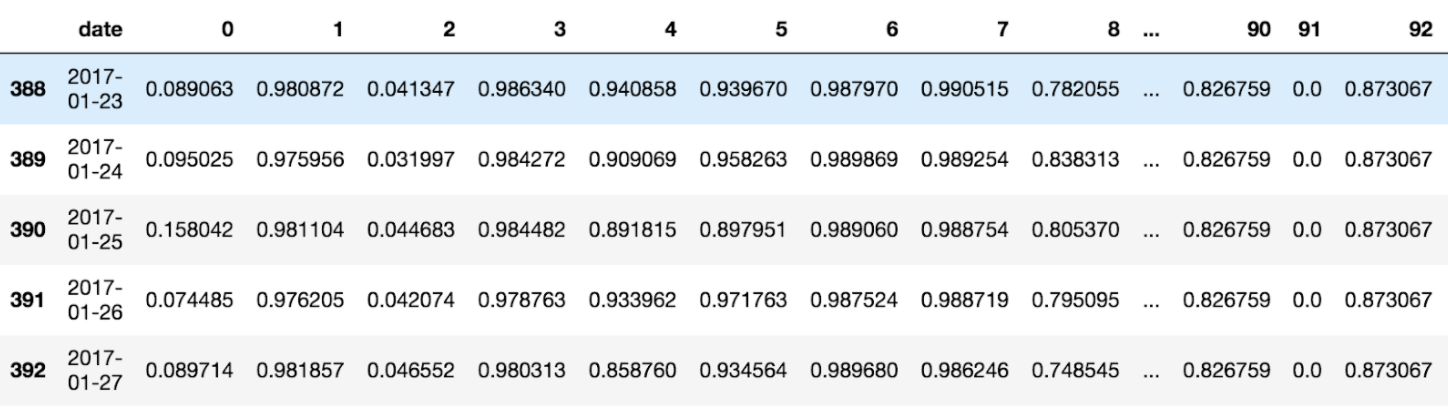
\includegraphics[width=\textwidth]{scaled.png}
\end{center}
\caption{Our input data, after being scaled.}
\end{figure}

\subsection{LSTM Architecture}

We used a Long Short Term Memory model to predict approval ratings. The LSTM took as input our preprocessed multivariate time series data (or moving averages of our multivariate time series data) and returned a predicted Trump approval rating for the next day. We used Keras' "Adam" optimizer, which is essentially a modified version of Stochastic Gradient Descent, and sought to minimize mean squared error on the data.

\subsection{Live news scraping}

In order to get live news results, we had to continuously scrape the web for news about Trump. To accomplish this, we built a scraper for Google News topics. Google News is an aggregator of news, such that the website does not actually write  its own news articles, rather, it maintains a feed of other newspapers, such as The New York Times and The Wall Street Journal. The Donald Trump topic on Google News is continuously updated with new articles.\\

Our scraper has minute resolution, such that every 60 seconds, it scans the provided HTML for updates. If there are new articles published, the scraper uses Beautiful Soup 4 to parse the HTML into Python, where we have to redirect it using Python's URL library. Links on Google News are in the form "https://news.google.com...", but we need the actual URL for the next step. Thus, we use the URL library to redirect links in the form "https://news.google.com..." to the actual article links, such as "www.npr.org/...". \\

Then, we use Python's News package, a downloadable package that makes article scraping easier. We feed the article URL obtained above, and using the package's methods, we are able to download the article title and body text in a matter of seconds. However, some news sites, such as Forbes, blocks anomalous HTTPs requests, such as those generated by our scraper bot, so therefore, we do not have total coverage of the news spectrum. However, we were still able to get good data by leaving our scraper on. \\

We ran our scraper for 71 hours, from 1 AM July 16th to 11 PM July 18th. In these 71 hours, we were able to scrape roughly 2,600 articles. In this time, there was a lot of turmoil in the country: federal agents in Portland, Mary Trump's book release, and more COVID-related closures in many states. Thus, we attribute the more-than-anticipated article volume to instability in the United States. 

\subsection{Results}

Our best-performing model (by MSE on our test dataset) utilized a stacked LSTM architecture, and we found that using 30-day moving averages minimized MSE. We hypothesize that this is due to the smoothing effect taking moving averages has on the data. However, in hindsight, using ARIMA instead of standard moving averages likely would have returned even better results.

\begin{figure}[H]
\begin{center}
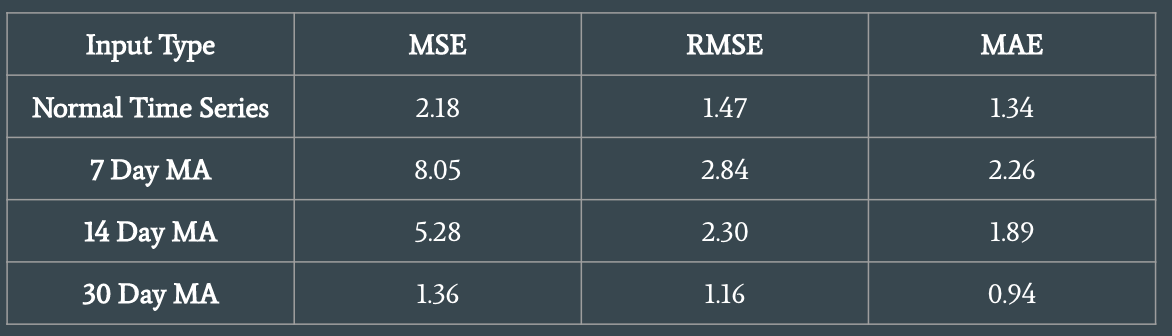
\includegraphics[width=\textwidth]{metrics.png}
\end{center}
\caption{Various test metrics over different types of input data, using a single LSTM.}
\end{figure}

Ultimately, we were able to achieve a Mean Squared Error of 1.30 and a Mean Average Error of 0.99 on our test data. While our model is far from perfect at predicting future approval ratings, 1.30 is far better relative to our previous models, we believe that further experimentation with different LSTM architectures could improve on this mark. 

\begin{figure}[H]
\begin{center}
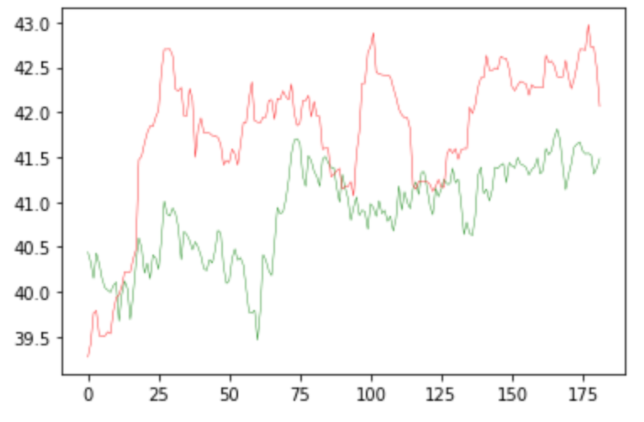
\includegraphics[width=\textwidth]{prediction.png}
\end{center}
\caption{Our predicted approval (green) and test approval (red) with our final stacked LSTM model.}
\end{figure}

\begin{figure}[H]
\begin{center}
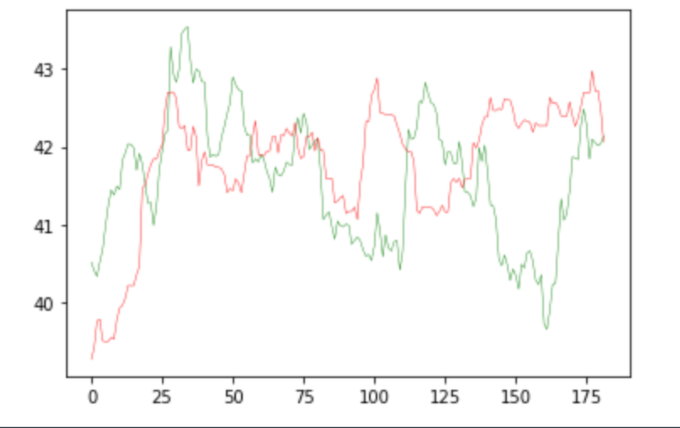
\includegraphics[width=\textwidth]{prediction_old.png}
\end{center}
\caption{Our predicted approval (green) and test approval (red) with a single LSTM model.}
\end{figure}

\section{Future Plans}

\subsection{Public Opinion Model}

Due to time constraints, we were only able to consider media opinion, while the original scope of our project considered media opinion relative to public opinion. If we choose to work on this project in our own time in the future, one direction we can take this project is by scraping discussion boards such as Reddit using a wrapper package such as PRAW. For instance, subreddits such as r/political-discussion have a high level of activity and frequently reference both Trump and Biden in their posts. One thing to be careful about with this approach, of course, is that we find a representative sample of public opinion, as many subreddits tend to skew conservative or liberal.

\subsection{Improvements to Model}

We believe that there is significant room for improvement in our LSTM. For instance, rather than using a simple moving average as input for our LSTM, we can utilize ARIMA (Autoregressive integrated moving average) before processing our input data. This would allow us to capture more information from our time series data, and hopefully better inform our LSTM. Our model could then use the change in approval rating (which is more stationary) as input and predict future daily changes in approval rating.

Additionally, higher resolution data would help us create more detailed time series for forecasting. Our approval rating data had only daily resolution, so switching to a different type of data or finding a better source for approval rating would help as well.

\end{document}
